%%%%%%%%%%%%%%%%%%%%%%%%%%%%%%%%%%%%%%%%%%%%%%%%%%%%%%%%%%%%%%%%%%%%%%
% LaTeX Template: Curriculum Vitae 
% Source: http://www.howtotex.com/
%%%%%%%%%%%%%%%%%%%%%%%%%%%%%%%%%%%%%%%%%%%%%%%%%%%%%%%%%%%%%%%%%%%%%%

\documentclass[paper=a4,fontsize=11pt]{scrartcl} % KOMA-article class
							
\usepackage[english]{babel}
\usepackage{graphicx}                    % Enable pdflatex
\usepackage[svgnames]{xcolor}            % Colors by their 'svgnames'
\usepackage{geometry}
	\textheight=650pt
\usepackage{url}
\usepackage{fontawesome}
\usepackage[export]{adjustbox}

\frenchspacing              % Better looking spacings after periods
\pagestyle{empty}           % No pagenumbers/headers/footers

%%% Custom sectioning (sectsty package)
%%% ------------------------------------------------------------
\usepackage{sectsty}

\sectionfont{%			            % Change font of \section command
	\usefont{OT1}{phv}{b}{n}%		% bch-b-n: CharterBT-Bold font
	\sectionrule{0pt}{0pt}{-5pt}{3pt}}

%%% Macros
%%% ------------------------------------------------------------
\newlength{\spacebox}
\settowidth{\spacebox}{8888888888}			% Box to align text
\newcommand{\sepspace}{\vspace*{1em}}		% Vertical space macro

\newcommand{\MyName}[1]{ % Name
		\Huge \usefont{OT1}{phv}{b}{n} \hfill #1
		\par \normalsize \normalfont}
		
\newcommand{\MySlogan}[1]{ % Slogan (optional)
		\large \usefont{OT1}{phv}{m}{n}\hfill \textit{#1}
		\par \normalsize \normalfont}

\newcommand{\NewPart}[1]{\section*{\uppercase{#1}}}

\newcommand{\PersonalEntry}[2]{
		\noindent\hangindent=0em\hangafter=0 % Indentation
		\parbox{\spacebox}{        % Box to align text
		\textit{#1}}		       % Entry name (birth, address, etc.)
		\hspace{2.5em} #2 \par}    % Entry value

\newcommand{\SkillsEntry}[2]{      % Same as \PersonalEntry
		\noindent\hangindent=0em\hangafter=0 % Indentation
		\parbox{\spacebox}{        % Box to align text
		\textit{#1}}			   % Entry name (birth, address, etc.)
		\hspace{2.5em} #2 \par}    % Entry value	

\newcommand{\EducationEntry}[4]{
		\noindent \textbf{#1} \hfill      % Study
		\colorbox{Black}{%
			\parbox{6em}{%
			\hfill\color{White}#2}} \par  % Duration
		\noindent \textit{#3} \par        % School
		\noindent\hangindent=2em\hangafter=0 \small #4 % Description
		\normalsize \par}

\newcommand{\WorkEntry}[4]{				  % Same as \EducationEntry
		\noindent \textbf{#1} \hfill      % Jobname
		\colorbox{Black}{\color{White}#2} \par  % Duration
		\noindent \textit{#3} \par              % Company
		\noindent\hangindent=2em\hangafter=0 \small #4 % Description
		\normalsize \par}

%%% ------------------------------------------------------------
\begin{document}

\begin{figure}
    \vspace*{60pt}
    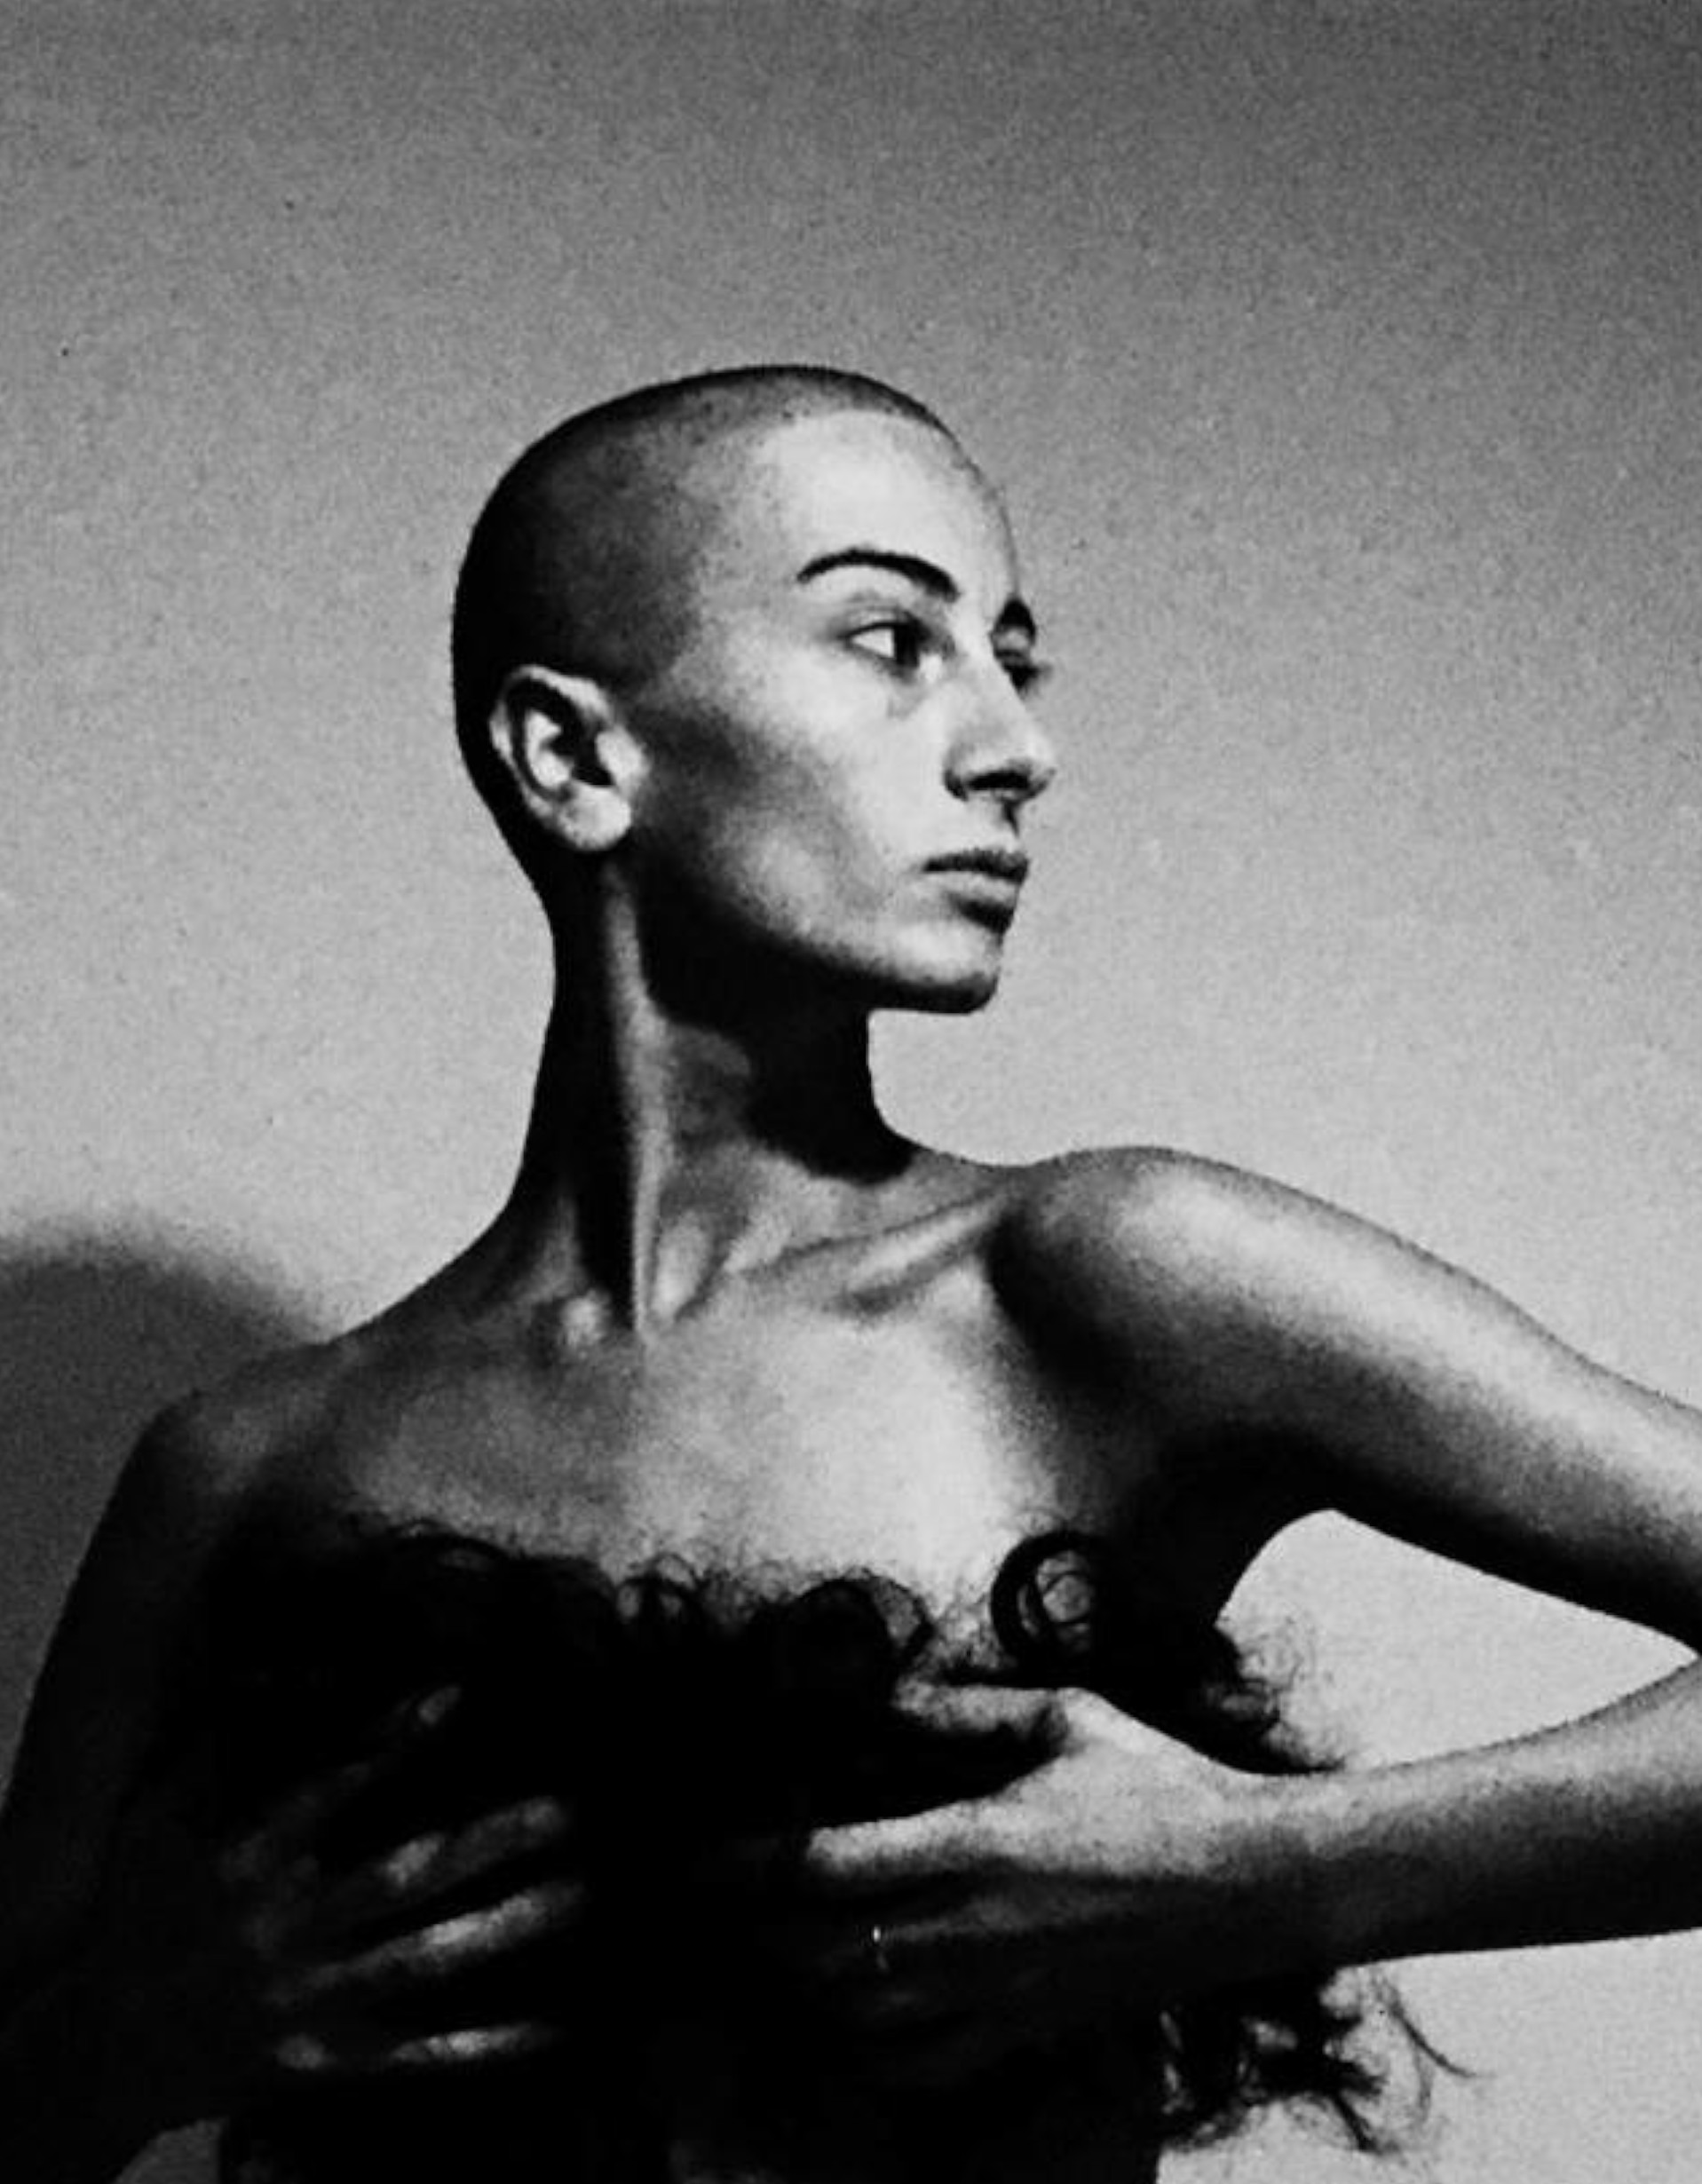
\includegraphics[width=1.1cm,left]{images/portrait}
    \vspace*{-30pt}
\end{figure}

\MyName{Simon Zimmermann}
\MySlogan{Curriculum Vitae}

\sepspace

%%% ------------------------------------------------------------
\NewPart{Personal details}{}

\PersonalEntry{Birth}{June 5, 1993}
\PersonalEntry{Location}{Düsseldorf, Germany}
\PersonalEntry{Mail}{\url{mail@simonzimmermann.com}}
\PersonalEntry{Github}{\faGithub\space\url{github.com/SimonZimmer}}

%%% ------------------------------------------------------------
\NewPart{Education}{}

\EducationEntry{MSc. Media Informatics}{2018-2020}{University Of Applied Sciences Düsseldorf}{Thesis title: 'Scalable Modelling of Room Acoustic Characteristics for AR-devices on the Basis of Visual Information Using Deep Learning' - honors degree}
\sepspace
\EducationEntry{MSc. Music Informatics}{2018}{University Of Music Karlsruhe}{Guest Semester}
\sepspace
\EducationEntry{BEng. Media Engineering}{2012-2017}{University Of Applied Sciences Düsseldorf}{Thesis title: 'A concept for implementing room acoustic material properties in the context of a 3D-audio engine'}
\newpage

%%% ------------------------------------------------------------
\NewPart{Work experience}{}

\EducationEntry{C++ Software Engineer}{2020-present}{Dear Reality GmbH, Full-time}{Full stack development of multiple realtime audio applications. Process follows the guidelines of the test-driven development philosophy, modern C++ and scrum.}
\sepspace
\EducationEntry{Researcher / QA Engineer (working student)}{2017-2020}{Dear Reality GmbH, Part-time}{Research and development of audio-DSP related prototypes, quality assurance and test automation development.}
\sepspace

\EducationEntry{Room-Acoustics Engineer (working student)}{2016-2017}{ISRW-Klapdor Part-time}{Room acoustic simulation and measurement.}

%%% ------------------------------------------------------------
\NewPart{Skills}{}

\SkillsEntry{Languages}{German (mother tongue)}
\SkillsEntry{}{English (fluent)}
\sepspace

\SkillsEntry{Technologies}{\textsc{C++14}}
\SkillsEntry{}{Python}
\SkillsEntry{}{MATLAB}
\SkillsEntry{}{CMake}
\SkillsEntry{}{git}
\SkillsEntry{}{docker}
\SkillsEntry{}{Jenkins}
\SkillsEntry{}{POSIX}
\SkillsEntry{}{vim}
\SkillsEntry{}{\LaTeX}
\sepspace

\SkillsEntry{Frameworks}{googletest}
\SkillsEntry{}{google-benchmark}
\SkillsEntry{}{JUCE}
\SkillsEntry{}{pybind11}
\SkillsEntry{}{flask}
\SkillsEntry{}{numpy/scipy}
\SkillsEntry{}{matplotlib}
\SkillsEntry{}{keras/tensorflow}
\sepspace

\SkillsEntry{Other}{Music Production}
\SkillsEntry{}{Modular Synthesizer}
\SkillsEntry{}{Esoteric Programming Lanuages (Orca, TidalCylces)}

\end{document}

